\documentclass{article}
\usepackage[utf8]{inputenc}
\usepackage{graphicx}
\usepackage{cleveref}
\usepackage{enumitem}
\usepackage{float}


\title{Mechanical Documentation}
\author{Group M213 Mechanical Team; Pender, L.W. (lwp26) and Hendricks, M.A. (mah237)}
\date{December 2022}

% To be confirmed that it requires the setspace package, try with and without.
\usepackage{setspace}

% Let top 85% of a page contain a figure
\renewcommand{\topfraction}{0.85}

% Default amount of minimum text on page (Set to 10%)
\renewcommand{\textfraction}{0.1}

% Only place figures by themselves if they take up more than 75% of the page
\renewcommand{\floatpagefraction}{0.75}

%zet de bladspiegel :
\setlength\paperwidth{20.999cm}\setlength\paperheight{29.699cm}\setlength\voffset{-1in}\setlength\hoffset{-1in}\setlength\topmargin{1.499cm}\setlength\headheight{12pt}\setlength\headsep{0cm}\setlength\footskip{1.131cm}\setlength\textheight{25cm}\setlength\oddsidemargin{2.499cm}\setlength\textwidth{16.5cm}

\begin{document}

\maketitle

\newpage

\section{Parts List}

\subsection{Standard Mechanical Parts used}

\begin{table}[h]
    \centering
    \begin{tabular}{|c|c|c|}
        \hline
        \textbf{Part} & \textbf{Quantity} & \textbf{Part No.} \\ \hline
        \hline
        M3 Socket Head Cap Screws & 14 & -\\
        \hline
        M4 Socket Head Cap Screws & 7 & -\\
        \hline
        12v Battery & 1 & -\\ 
        \hline
        4” Wheel Vex 276-1497 & 2 & RP 70-6239\\
        \hline
        Ball Caster & 1 & -\\
        \hline
        Wheel Adaptors & 2 & -\\
        \hline
        18RPM 12v motor & 2 & OC 3999920\\
        \hline
        Standard Servo & 1 & MC-410 \\
        \hline
        Arduino wifi v2 & 1 & - \\
        \hline
        Adafruit Motor Shield V2 & 1 & - \\
        \hline
        Red Push Button & 1 & RP 78-0100\\
        \hline
        Ultrasonic sensor & 2 & HC-SR504\\
        \hline
        \textbf{Total} & 33 & -\\ \hline
    \end{tabular}
    \caption{Given Parts}
    \label{tab:given_parts}
\end{table}


\subsection{Manufactured Parts list}
% table of parts
\begin{table}[h]
    \centering
    \begin{tabular}{|c|c|c|c|}
        \hline
        \textbf{Part} & \textbf{Quantity} & \textbf{Manufacuring} \\ \hline
        \hline
        Top Plate & 1 & Laser Cut \\
        \hline
        Bottom Plate & 1 & Laser Cut \\
        \hline
        Bulkhead & 1 & Laser Cut \\
        \hline
        Castor Spacer & 1 & Laser Cut \\
        \hline
        Finger connector & 2 & Laser Cut \\
        \hline
        Left finger connector & 1 & Laser Cut \\
        \hline
        Right finger connector & 1 & Laser Cut \\
        \hline
        Grabber finger & 2 & Laser Cut \\
        \hline
        Front Ultrasonic mount & 1 & 3D printed \\
        \hline
        Top Connector & 1 & Sheet metal \\
        \hline
        Grabber & 2 & Sheet metal \\
        \hline
        Side ultrasonic mount & 1 & Sheet metal \\
        \hline
        Motor mount & 2 & Sheet metal \\
        \hline
        \textbf{Total} & 17 & \\ \hline
    \end{tabular}
    \caption{Manufactured Parts}
    \label{tab:manufactured_parts}
\end{table}

\section{Drawings}

\begin{figure}[H]
    \centering
    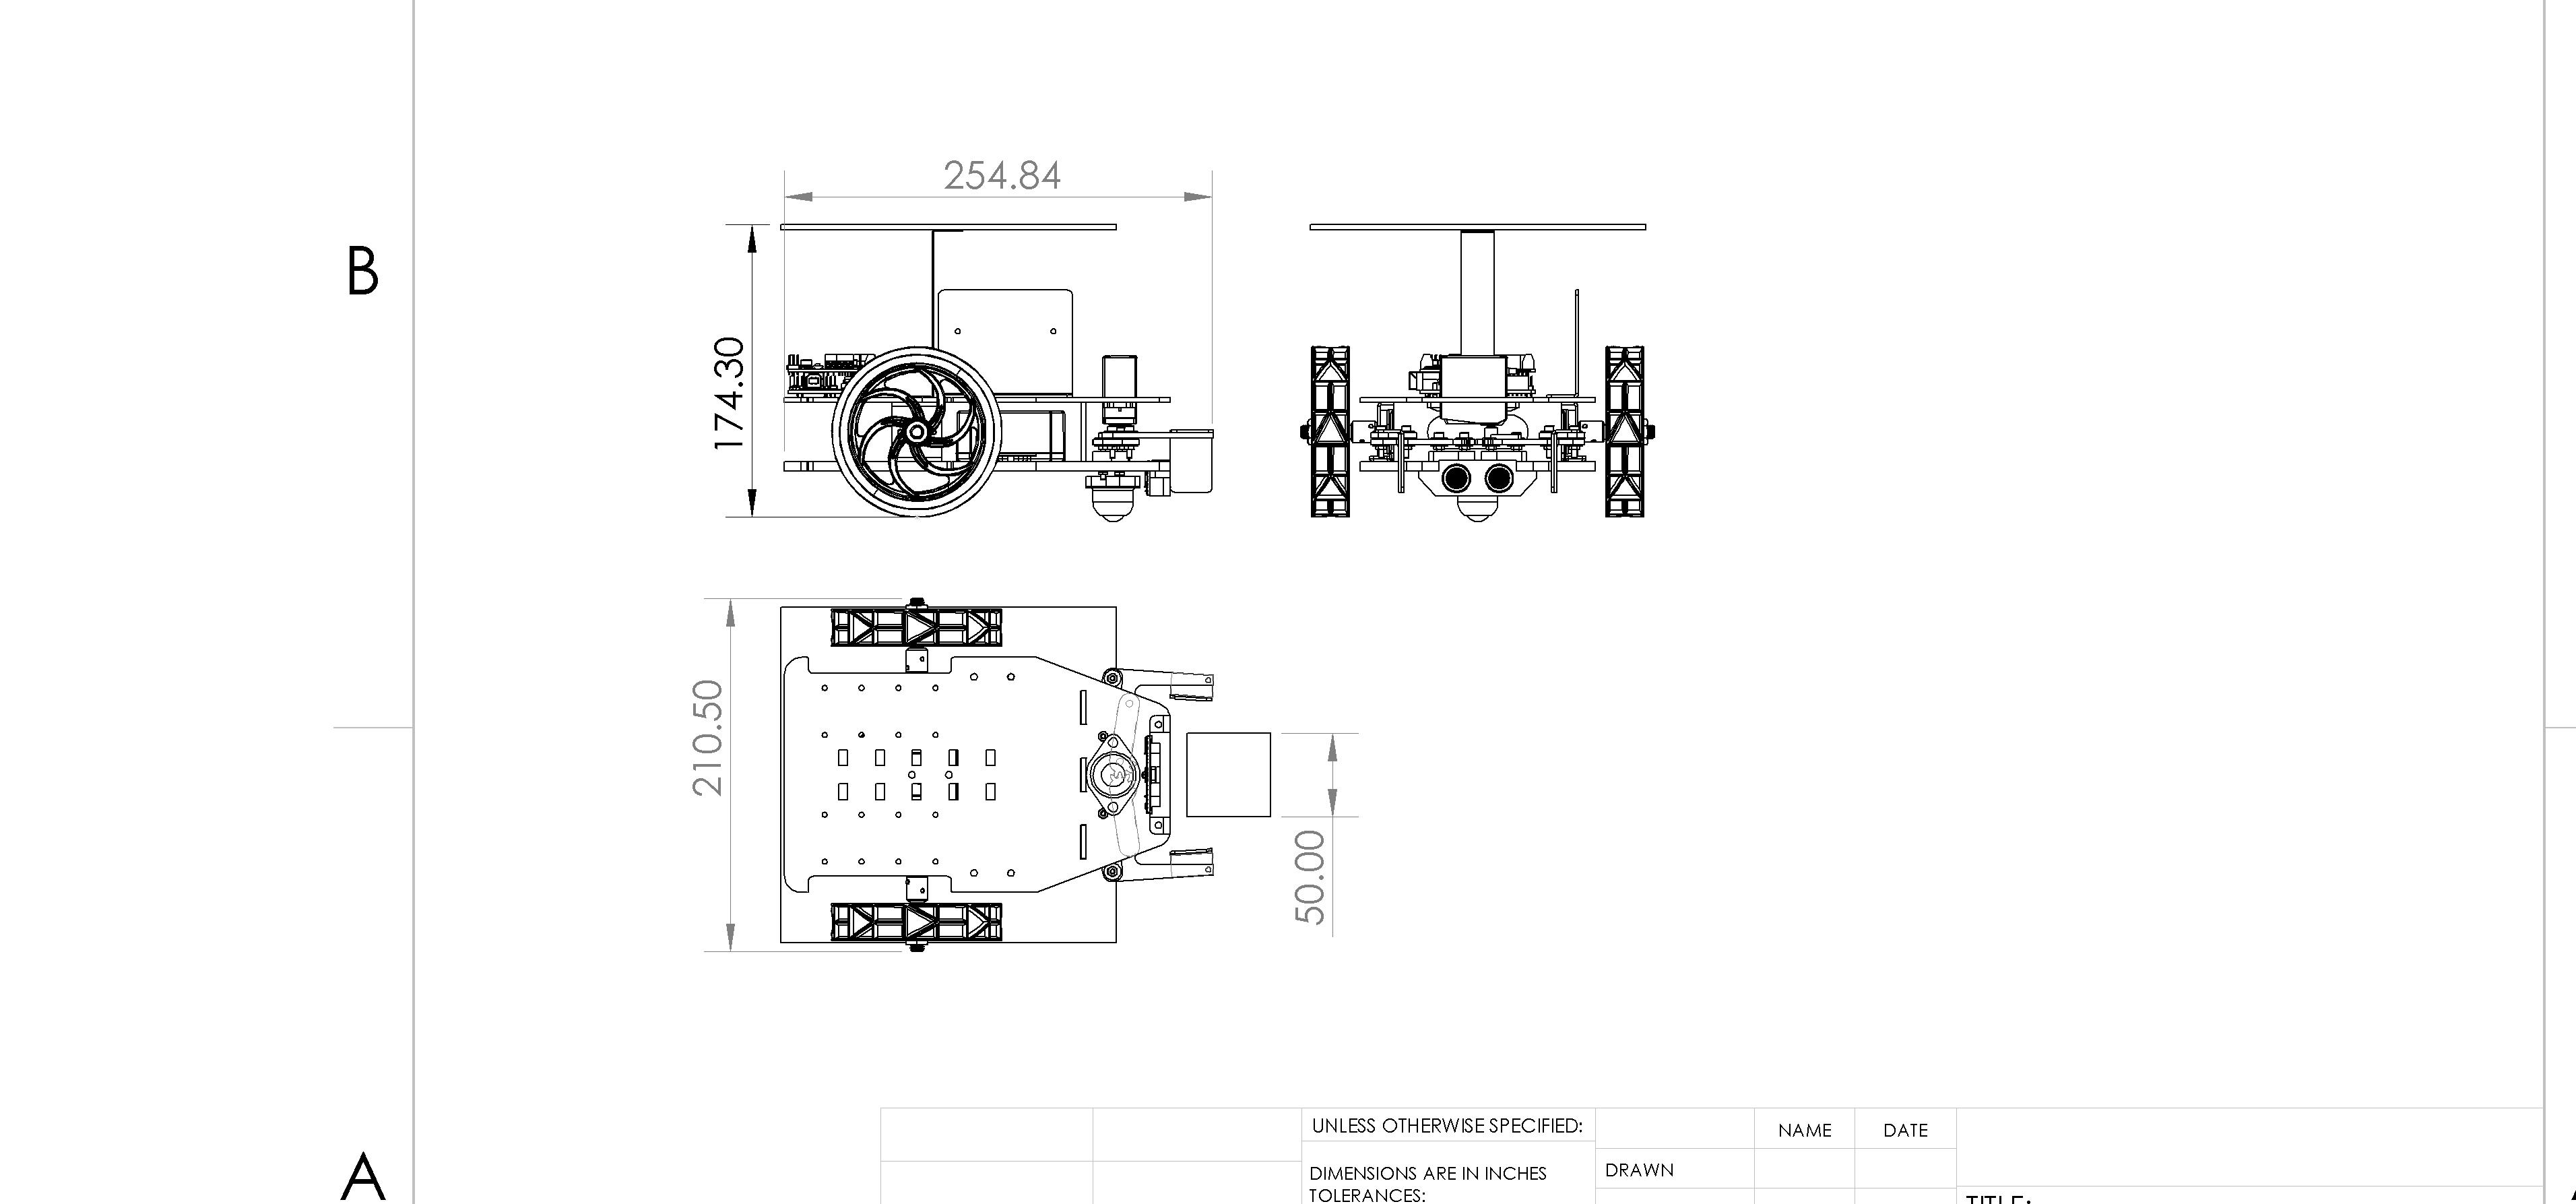
\includegraphics[width=0.8\textwidth]{assets/entire_model_drawing.JPG}
    \label{fig:entire_model_drawing}
    \caption{Drawing of entire robot}
\end{figure}

\begin{figure}[H]
    \centering
    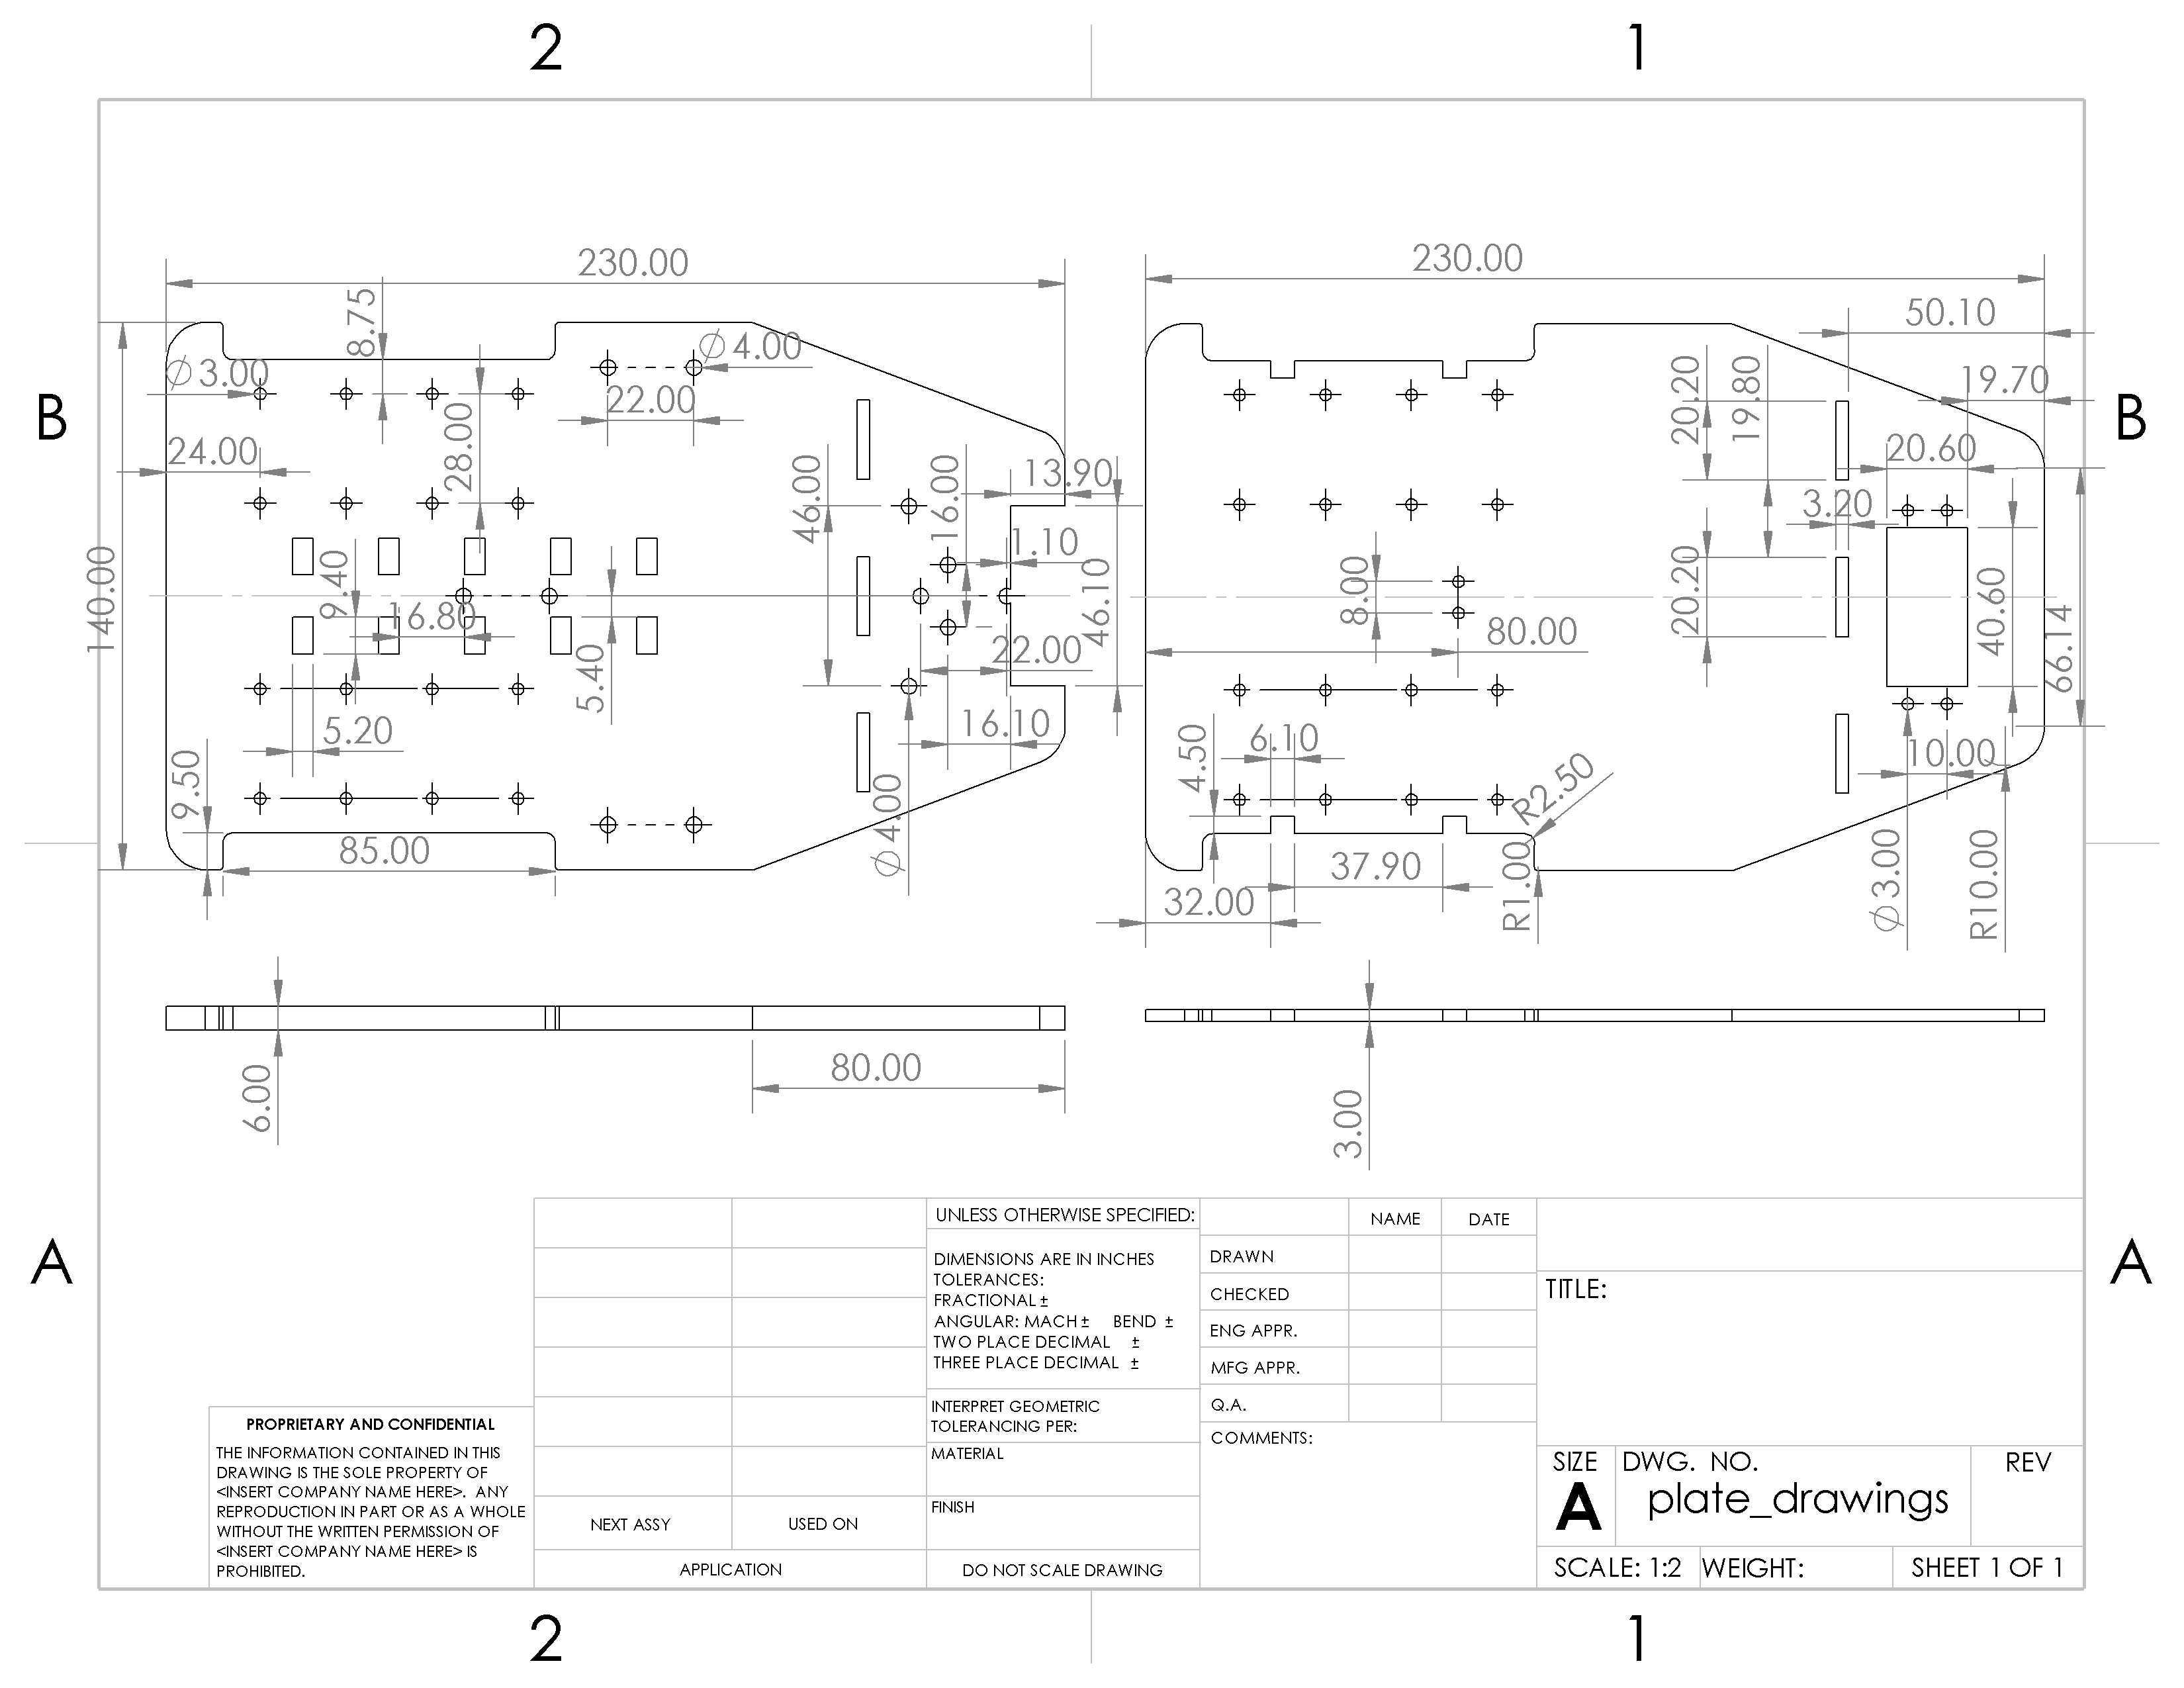
\includegraphics[width=0.8\textwidth]{assets/plate_drawings.JPG}
    \label{fig:plate_drawings}
    \caption{Drawing of upper and lower plates}
\end{figure}

\begin{figure}[H]
    \centering
    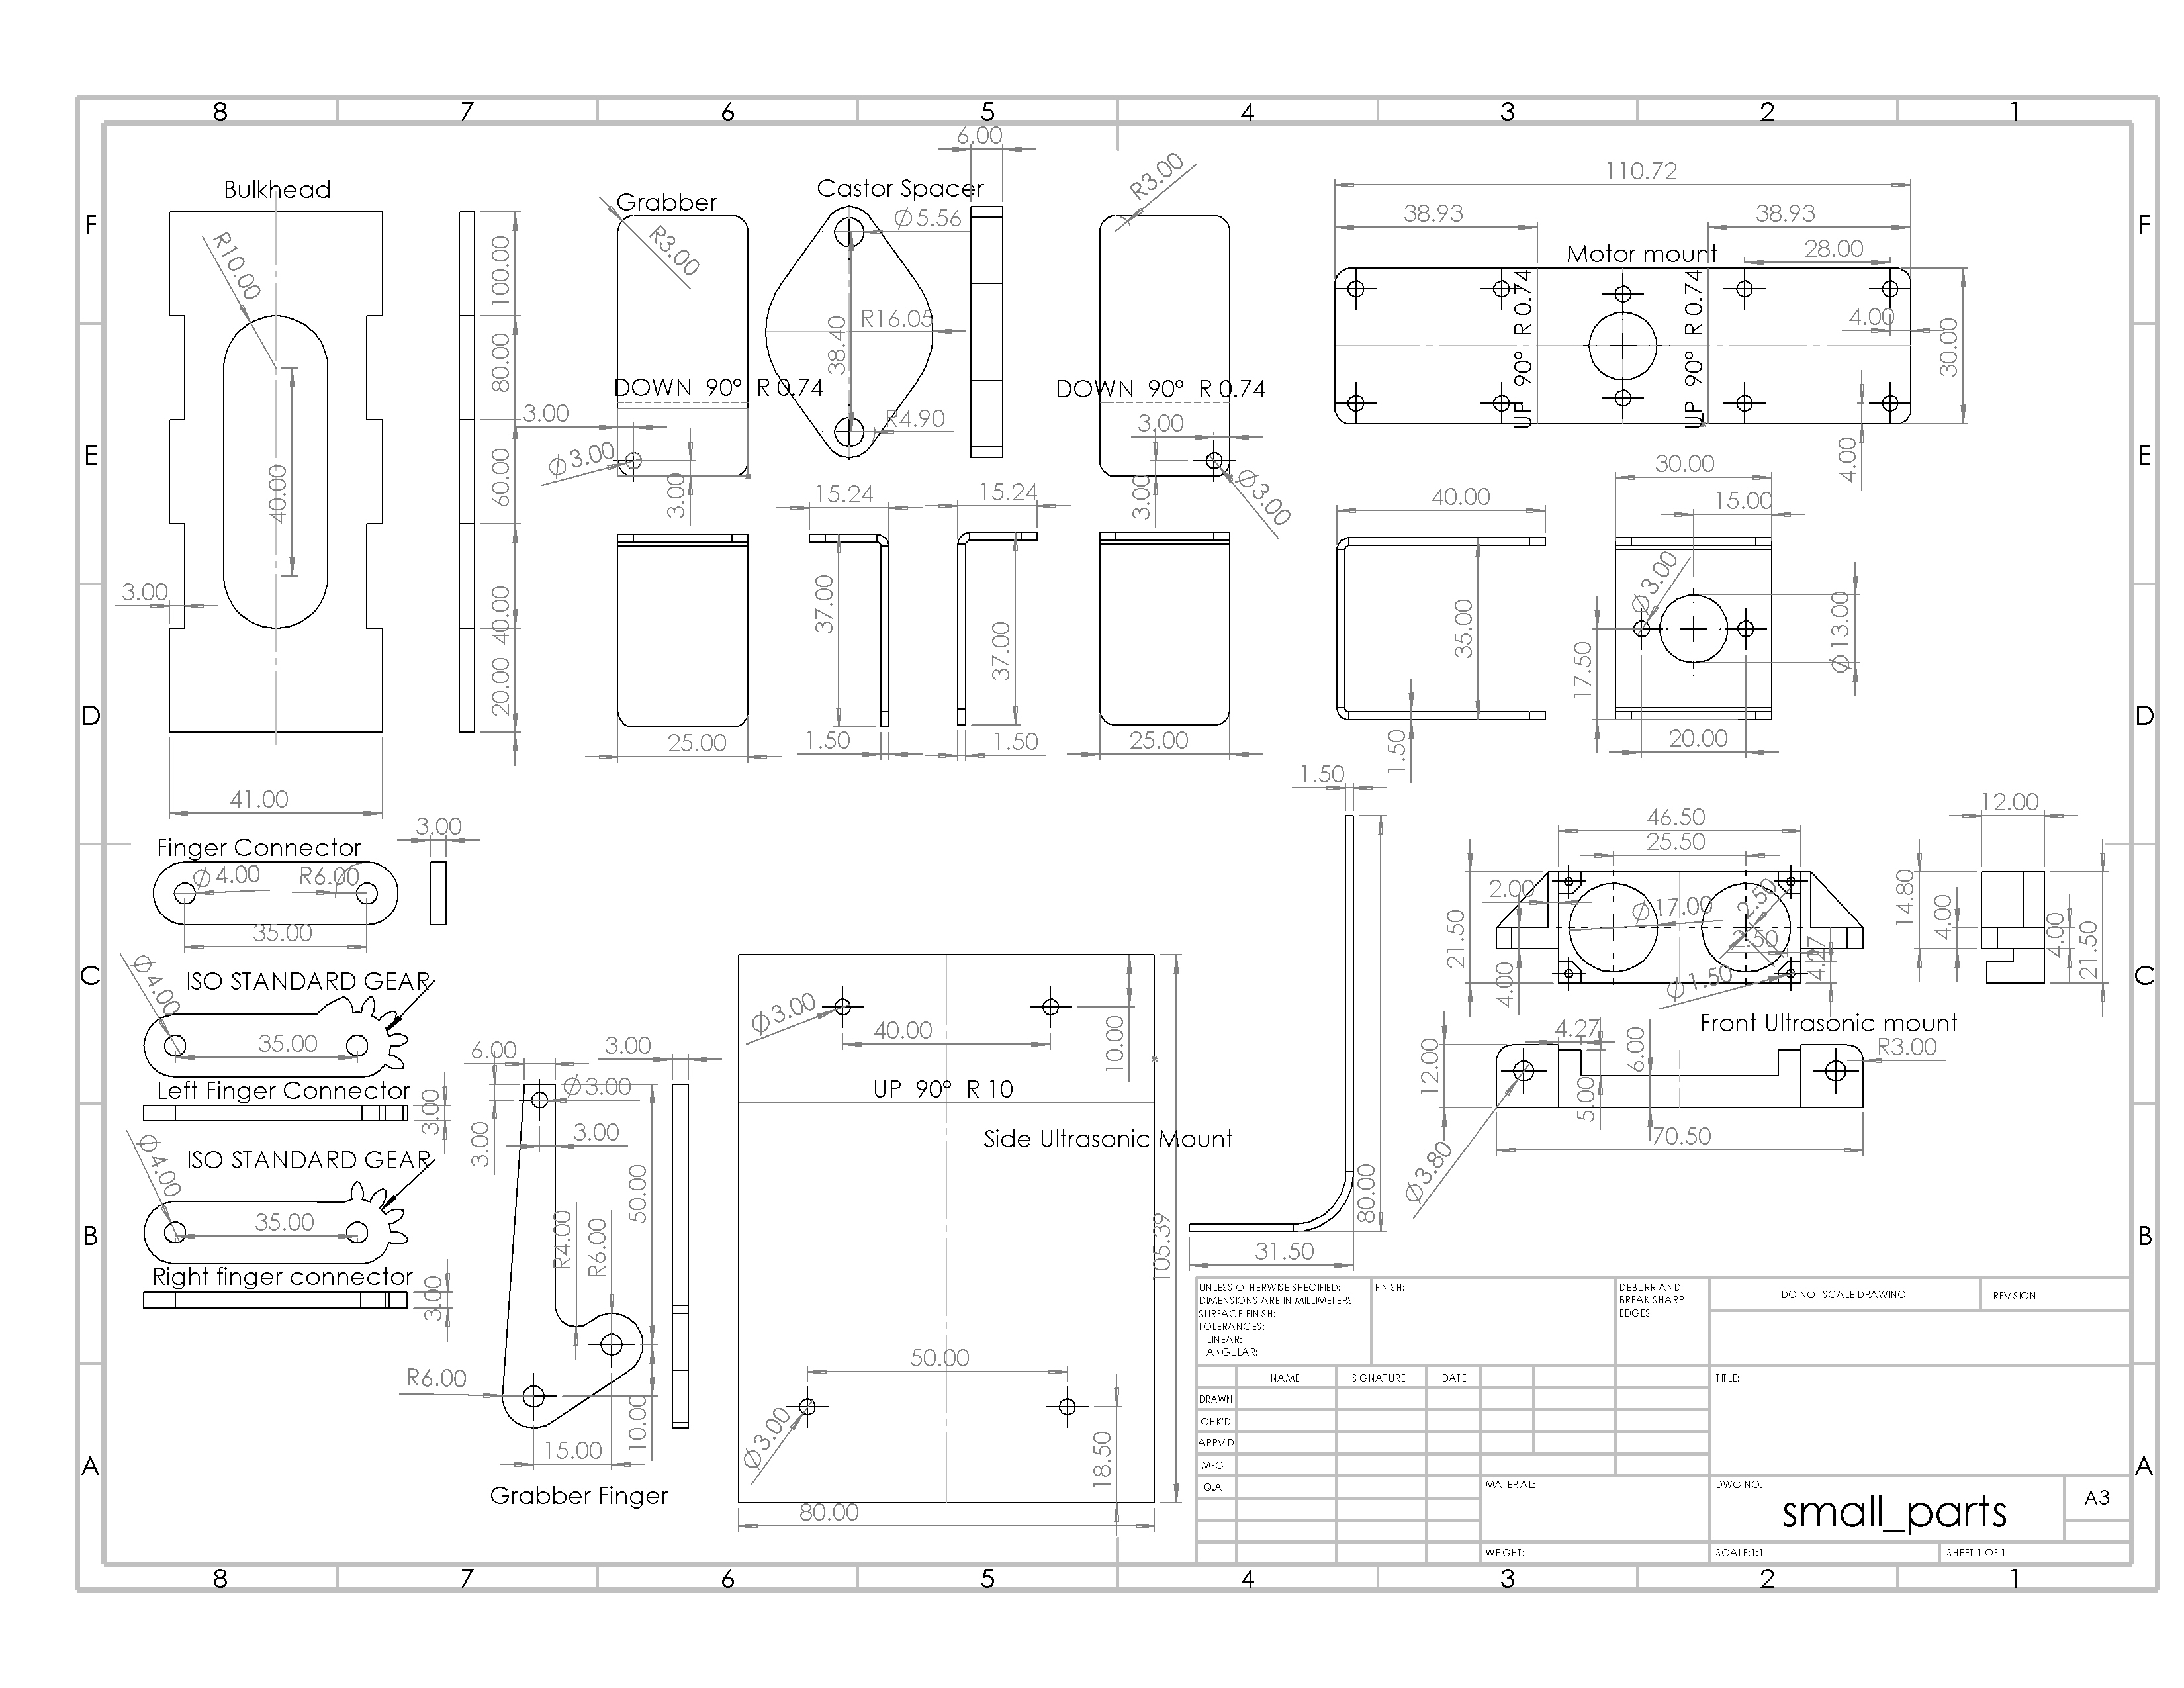
\includegraphics[width=0.8\textwidth]{assets/small_parts.JPG}
    \label{fig:smaller_parts}
    \caption{Drawing of smaller parts}
\end{figure}

\section{Manufacuring}

\subsection{Laser cut parts}
\quad As shown in the parts list, we mostly used laser cut parts. The parts were cut from sheets of 3mm or 6mm laser ply. The laser has a diameter of 0.2mm and so has a tolerance of 0.1mm which was accuate enough that we did not need to account for in our design. Most of the laser cut parts were hot glued together but bolted elsewhere.

\subsection{Sheet metal parts}
\quad The sheet metal parts were cut from 1.5mm steel sheet. The parts were cut using a guillotine and then bent using a manual bender. The metal parts all attached to the chassis by nuts and bolts.

\section{Assembly}
\quad The robots mechanical parts were assembled using nuts, hex bolts and washers. Electrical parts were attached later using zip ties. The LED and LDR are omitted from CAD but were attached using a single bolt and some additional hot glue.

\subsection {Chassis}

\subsection{Gripping Mechanism}
\quad The gripping mechanism designed made it very difficult to assemble however the assembly order can be seen in the following ordered images.

\subsubsection{Bottom gripping mechanism section assembly} 

\begin{figure}[H]
    \centering
    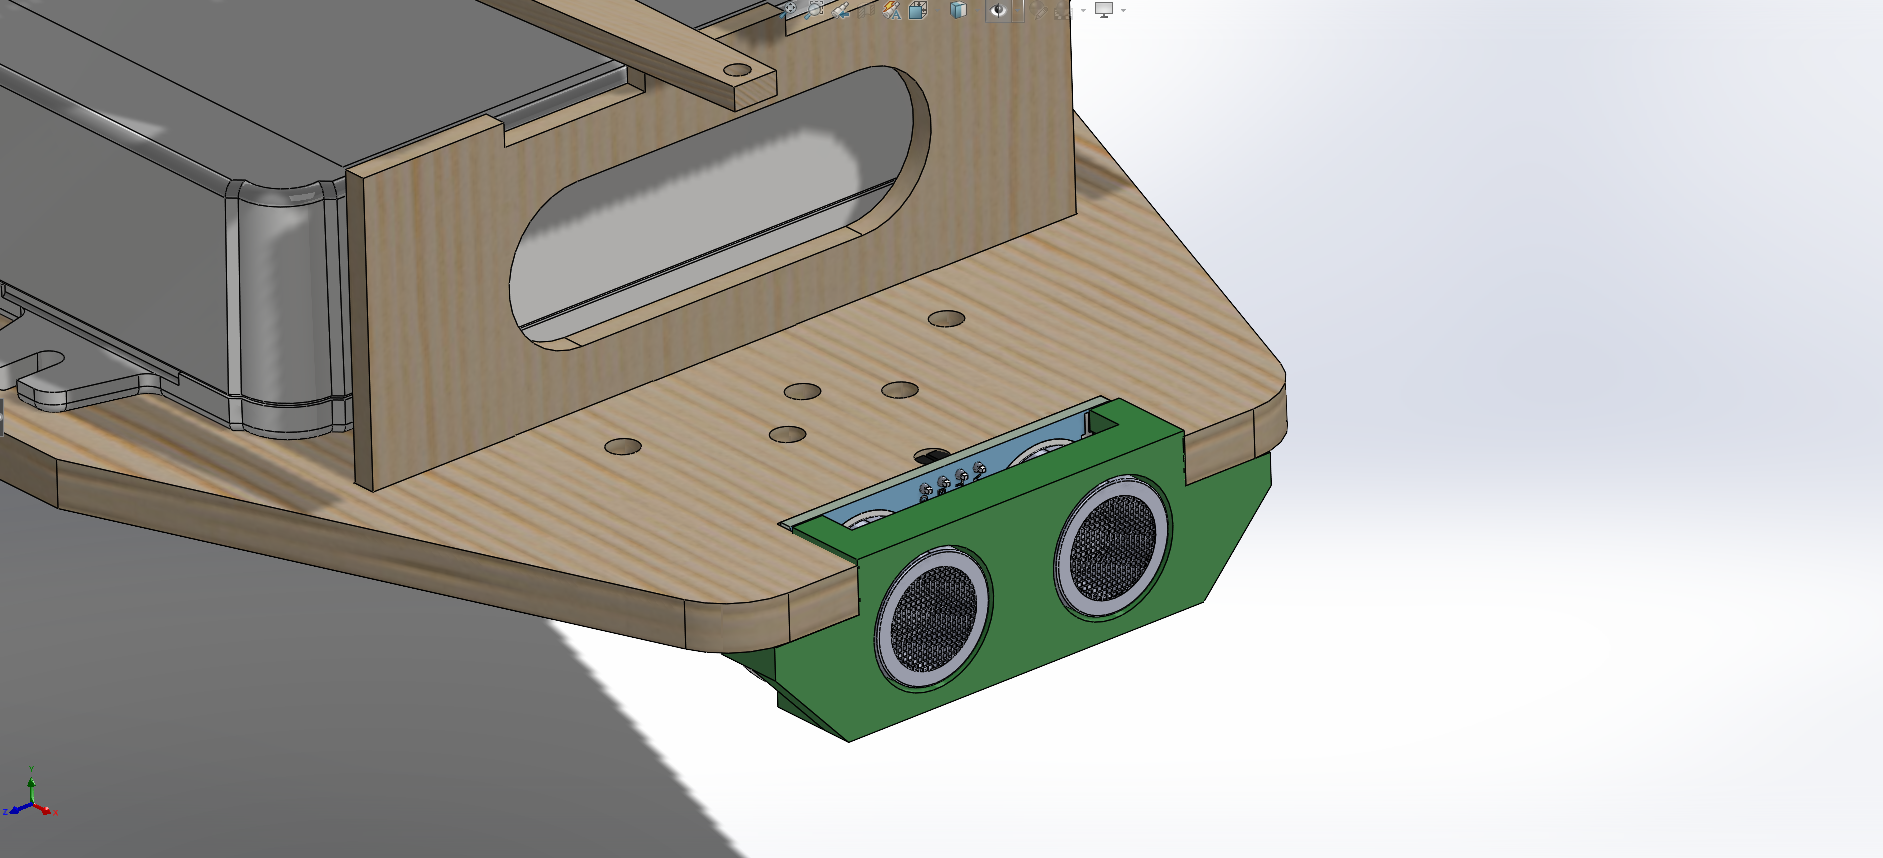
\includegraphics[width=0.8\textwidth]{assets/assembly/1.png}
\end{figure}

\begin{figure}[H]
    \centering
    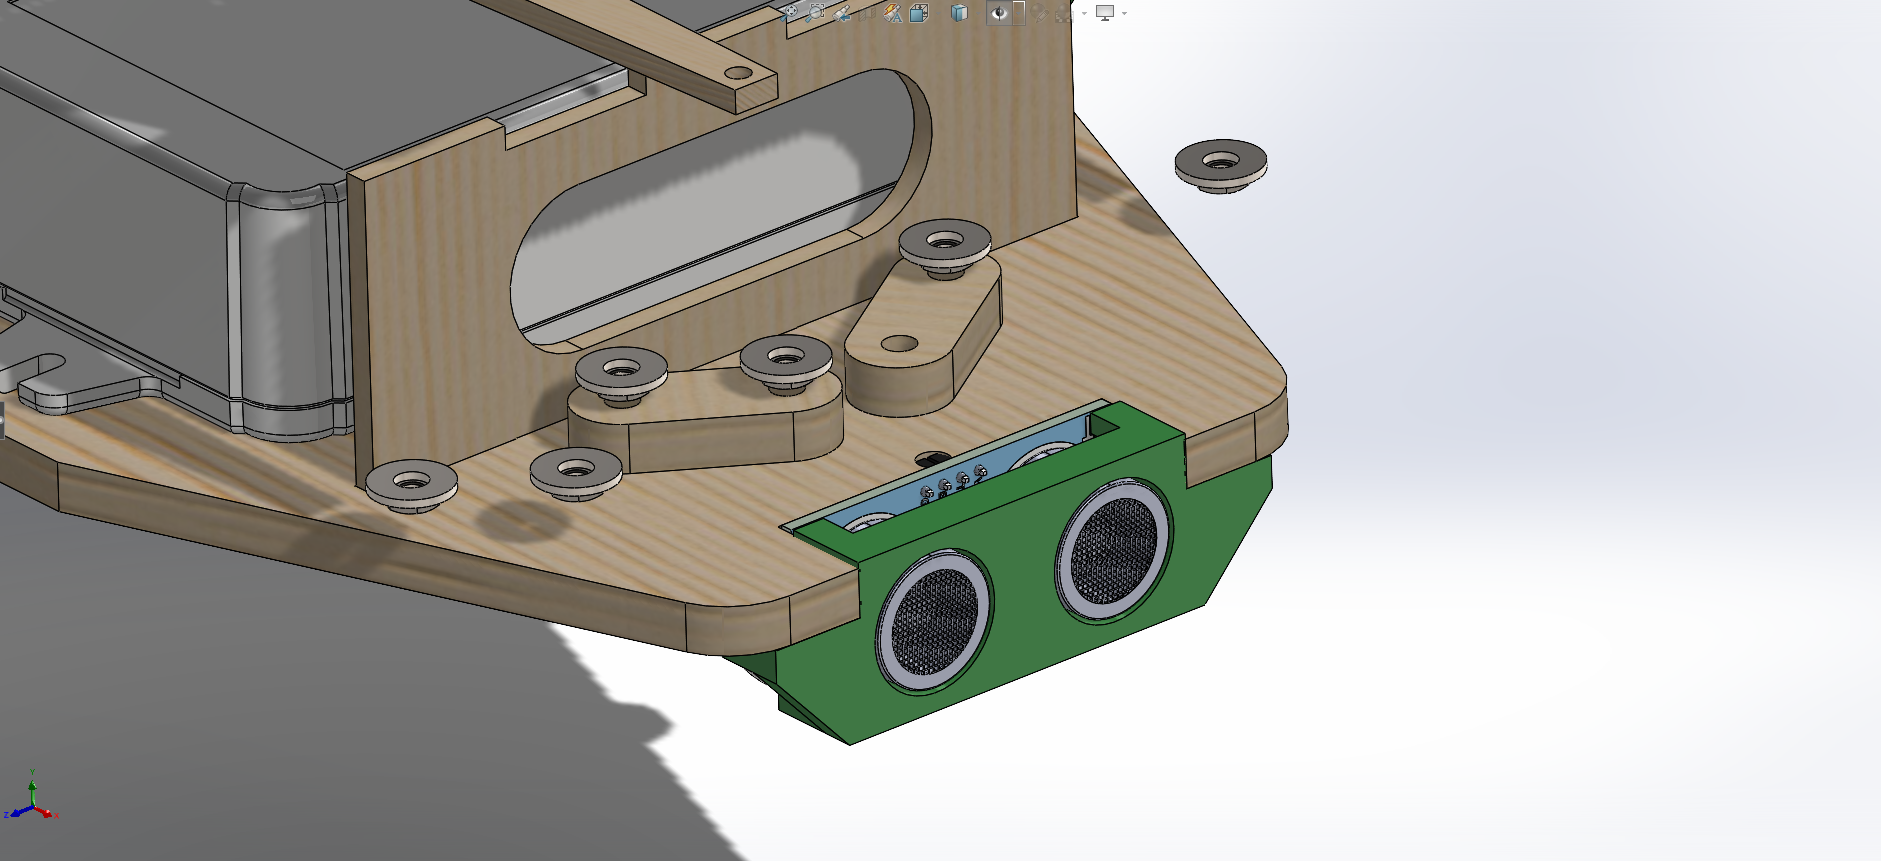
\includegraphics[width=0.8\textwidth]{assets/assembly/2.png}
\end{figure}

\begin{figure}[H]
    \centering
    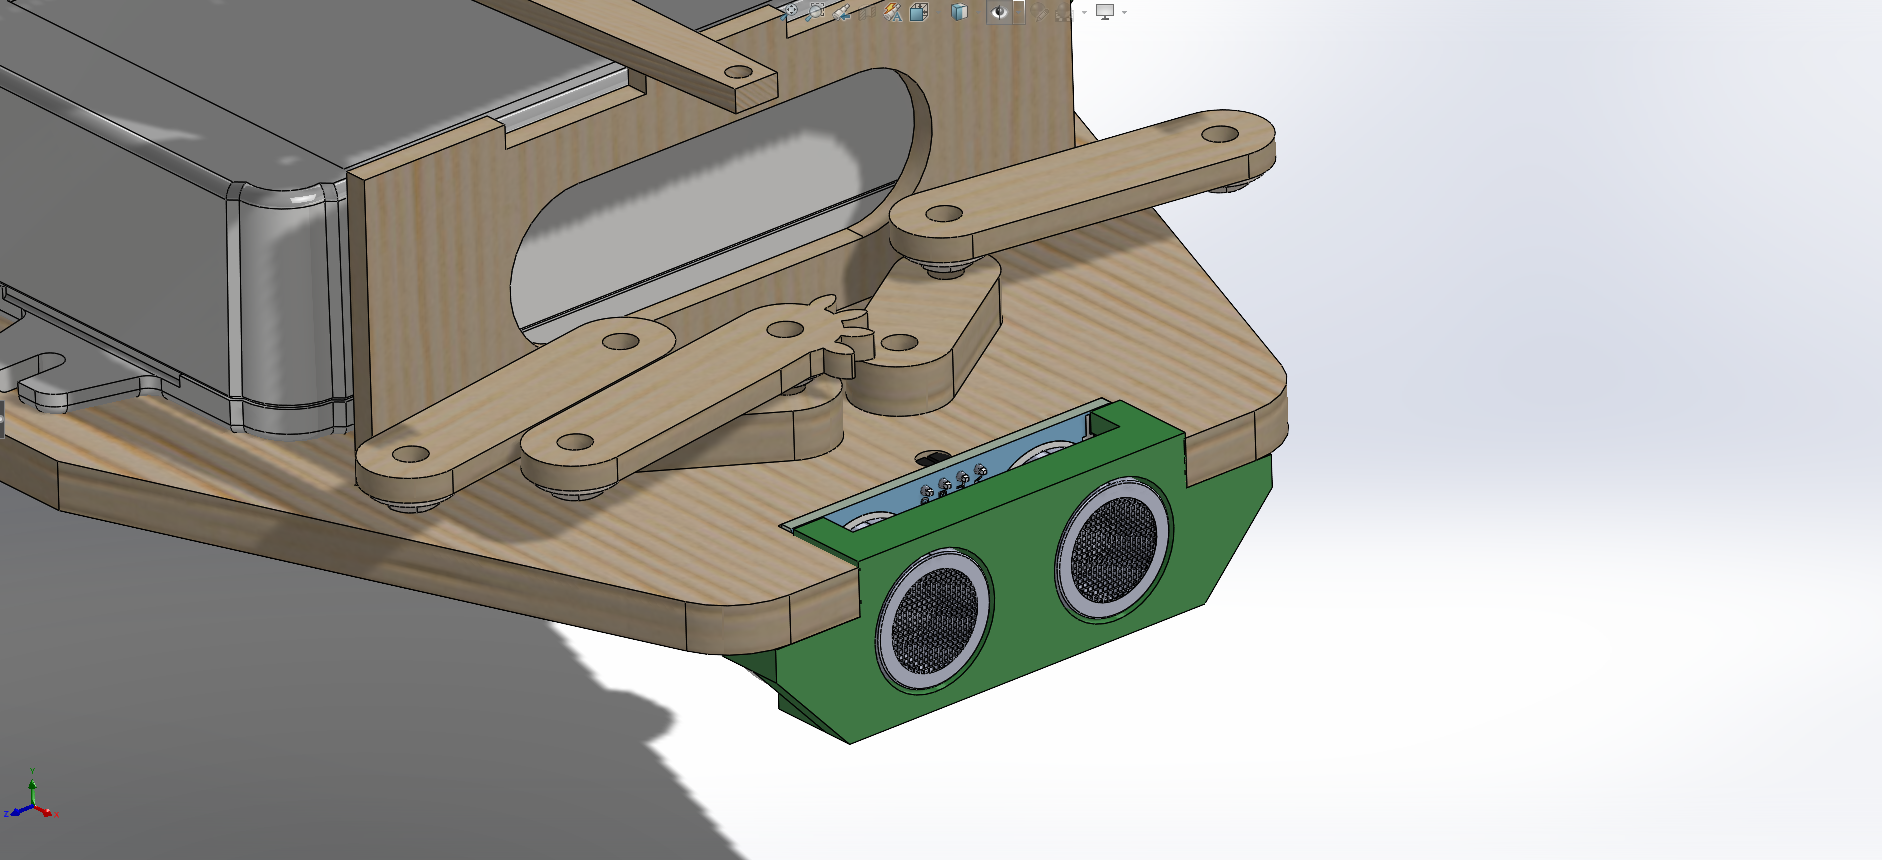
\includegraphics[width=0.8\textwidth]{assets/assembly/3.png}
\end{figure}

\begin{figure}[H]
    \centering
    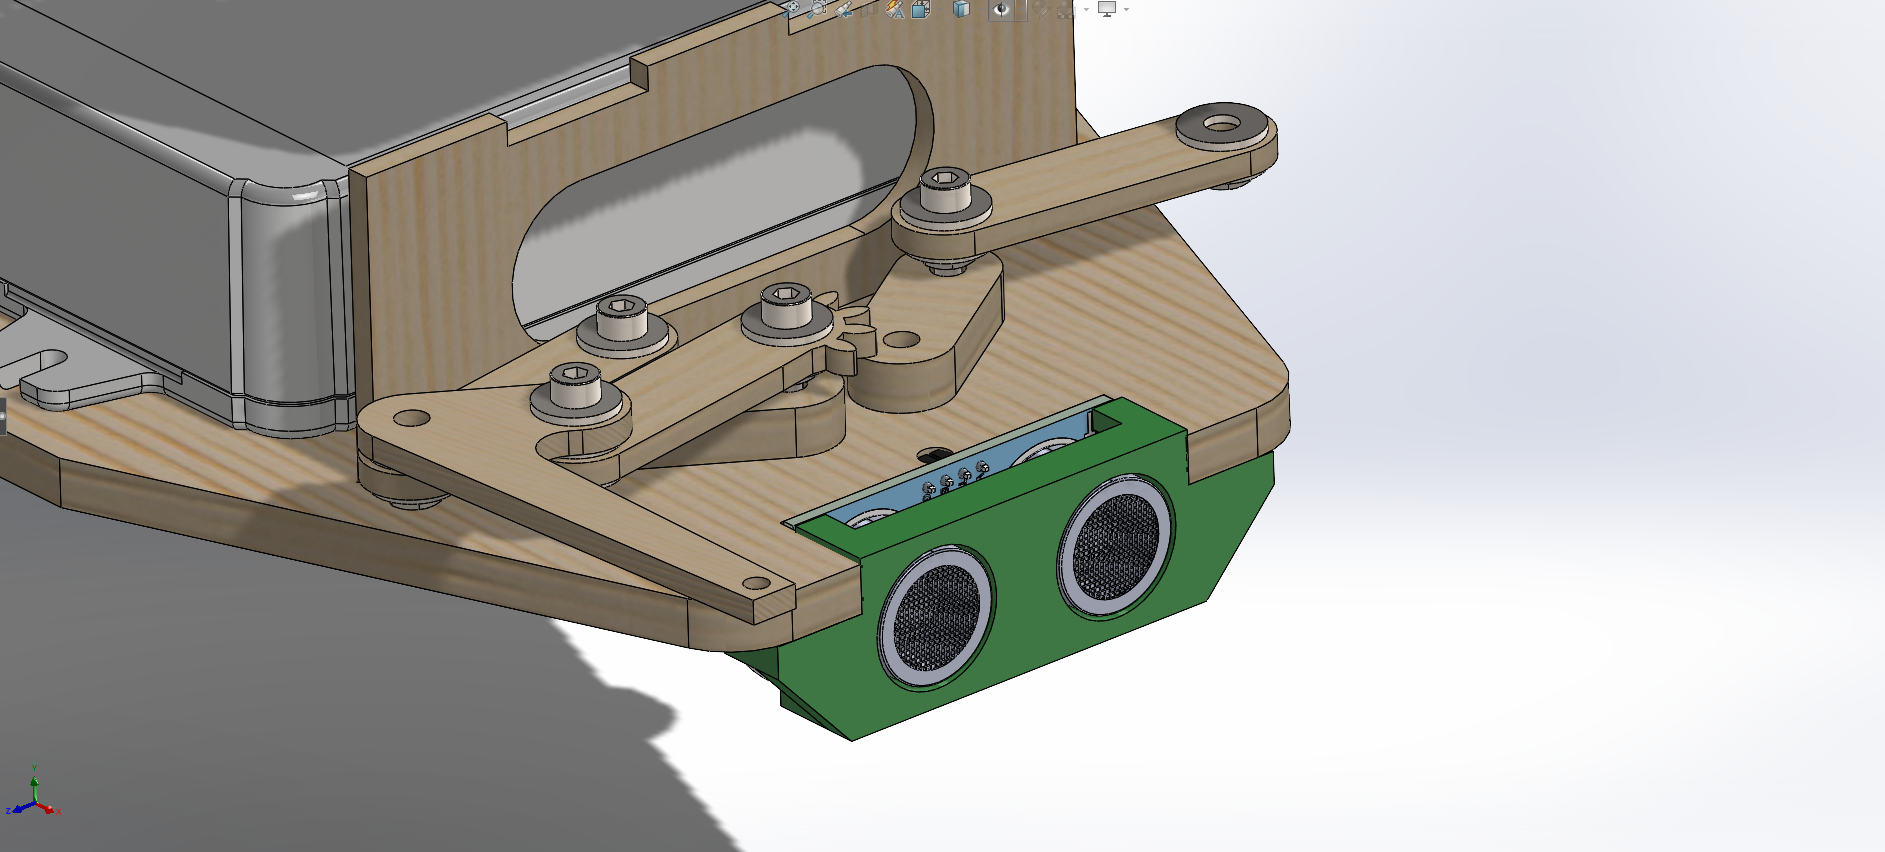
\includegraphics[width=0.8\textwidth]{assets/assembly/4.png}
\end{figure}

\subsubsection{Top gripping mechanism section assembly} 

\begin{figure}[H]
    \centering
    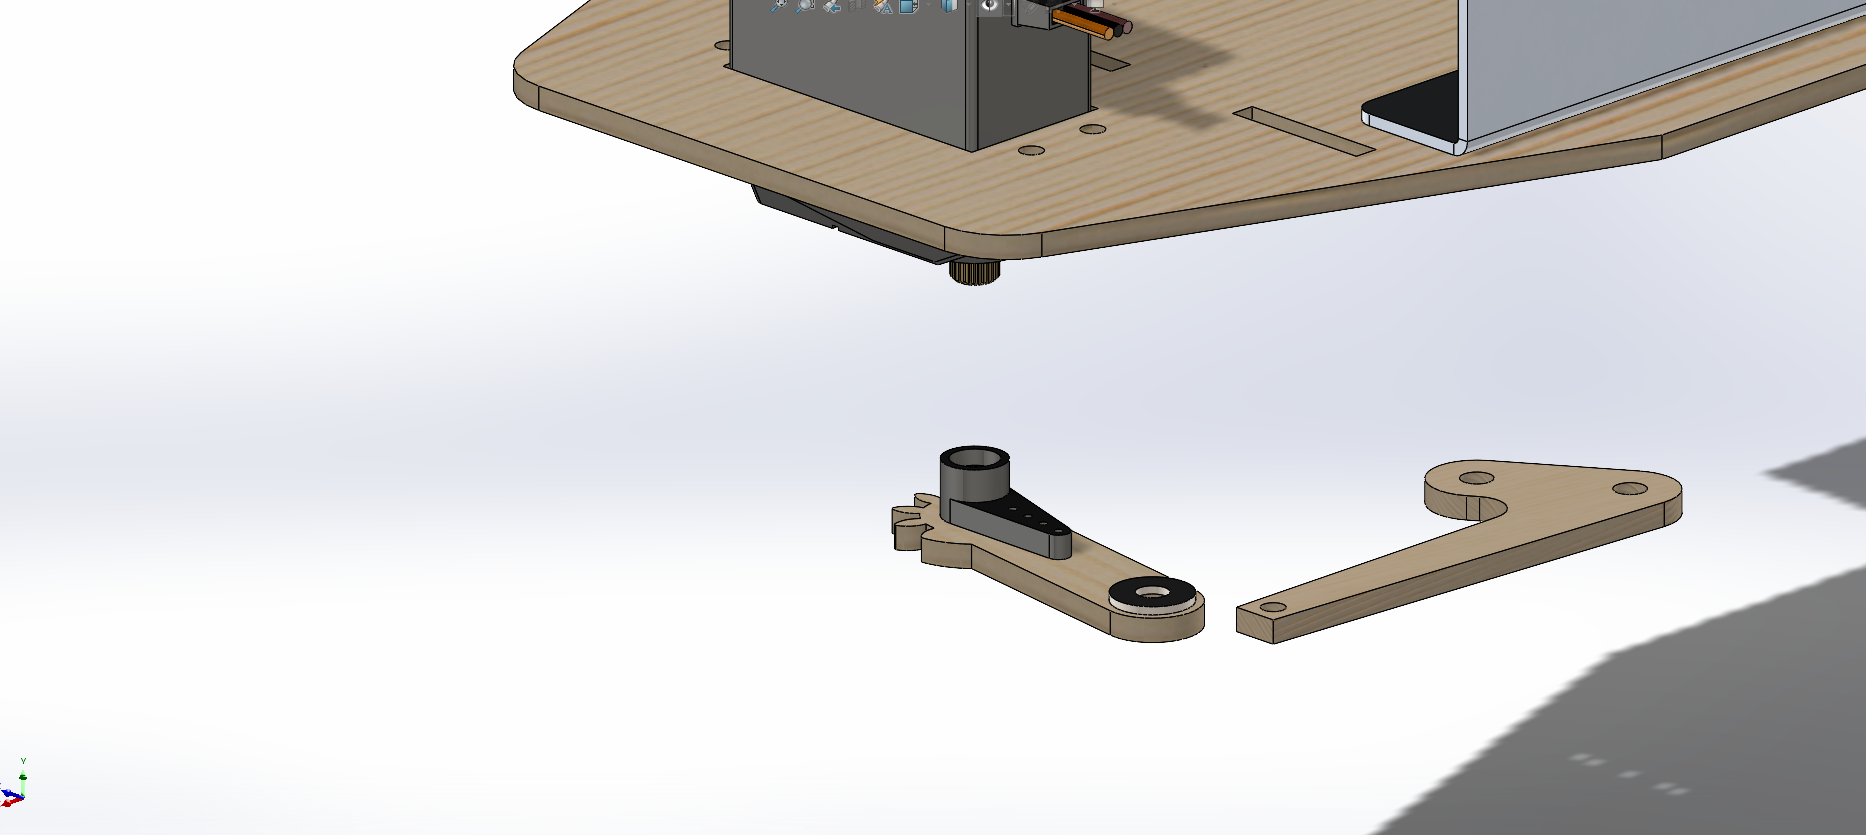
\includegraphics[width=0.8\textwidth]{assets/assembly/5.png}
\end{figure}

\begin{figure}[H]
    \centering
    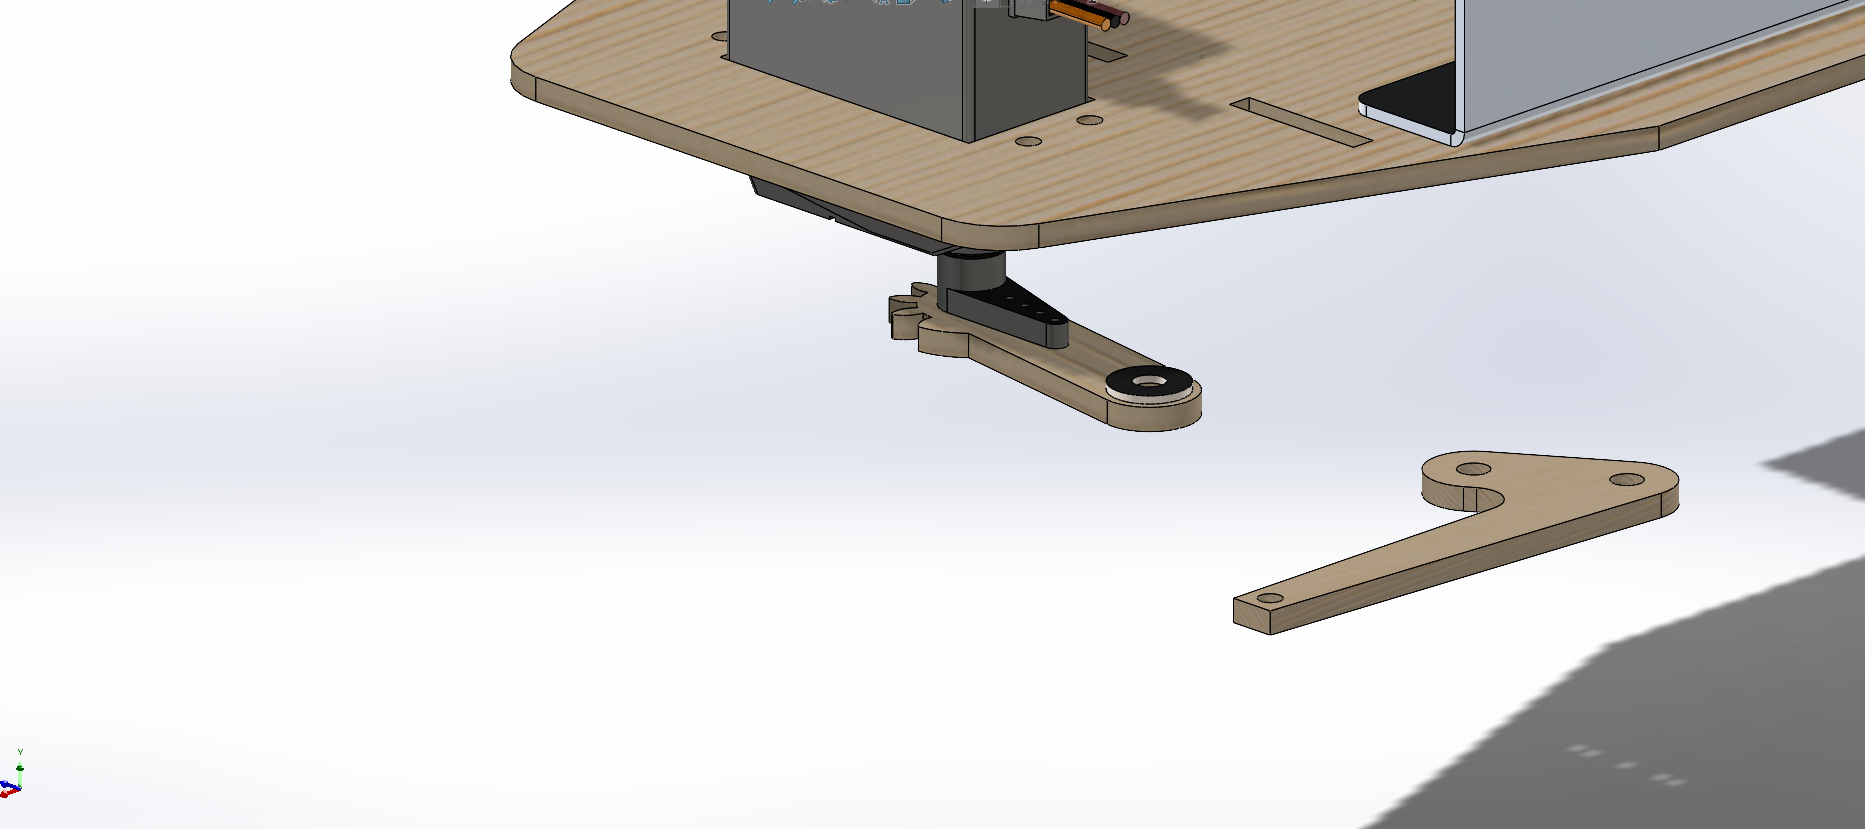
\includegraphics[width=0.8\textwidth]{assets/assembly/6.png}
\end{figure}

\begin{figure}[H]
    \centering
    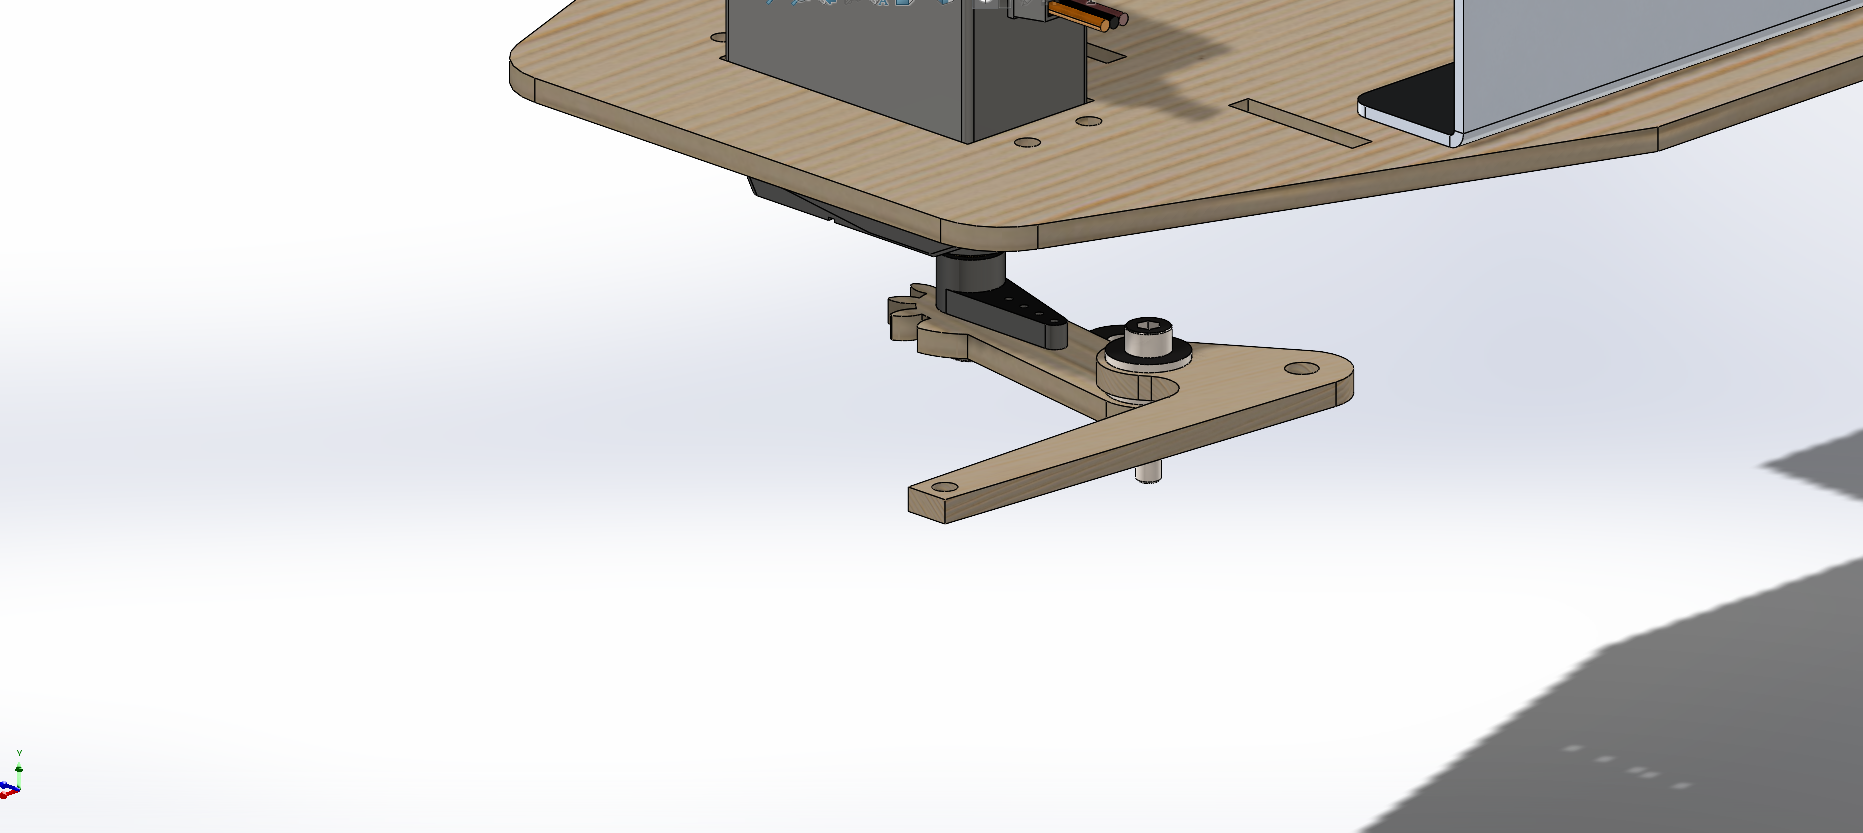
\includegraphics[width=0.8\textwidth]{assets/assembly/7.png}
\end{figure}

\subsubsection{Top and bottom section assembly}
\quad Note that it is important that the gears mesh correctly such that the grabber can be opened and closed. 

\begin{figure}[H]
    \centering
    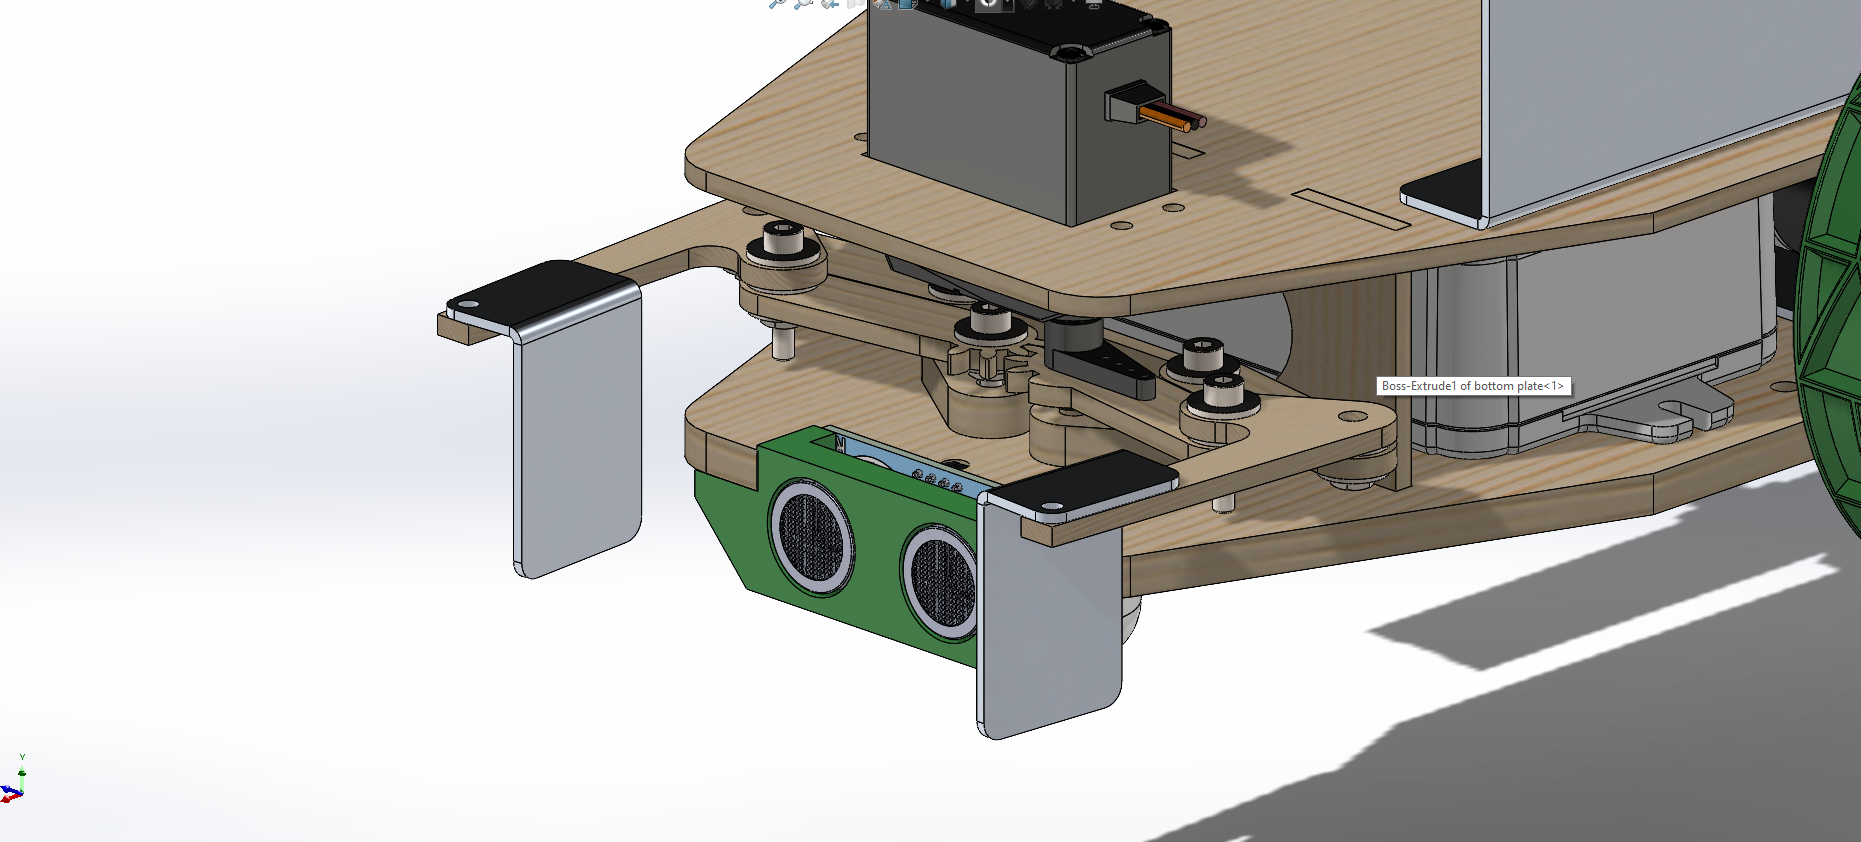
\includegraphics[width=0.8\textwidth]{assets/assembly/8.png}
\end{figure}

\begin{figure}[H]
    \centering
    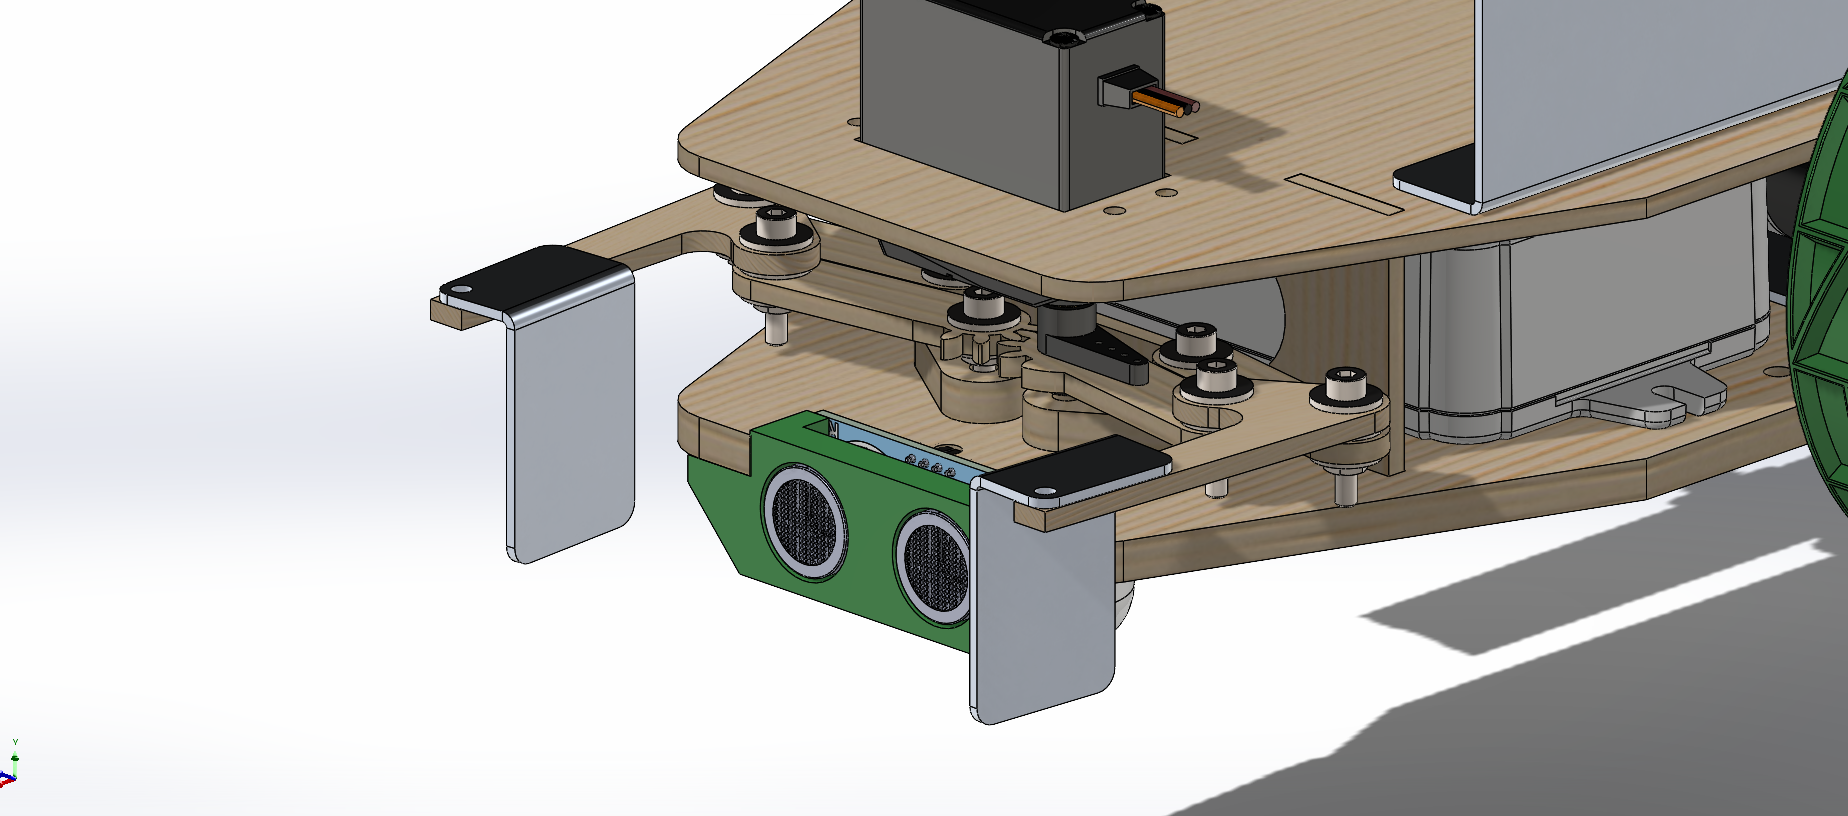
\includegraphics[width=0.8\textwidth]{assets/assembly/9.png}
    \caption{Fully assembled gripping mechanism}
\end{figure}

\section{CAD renders}

\begin{figure}[H]
    \centering
    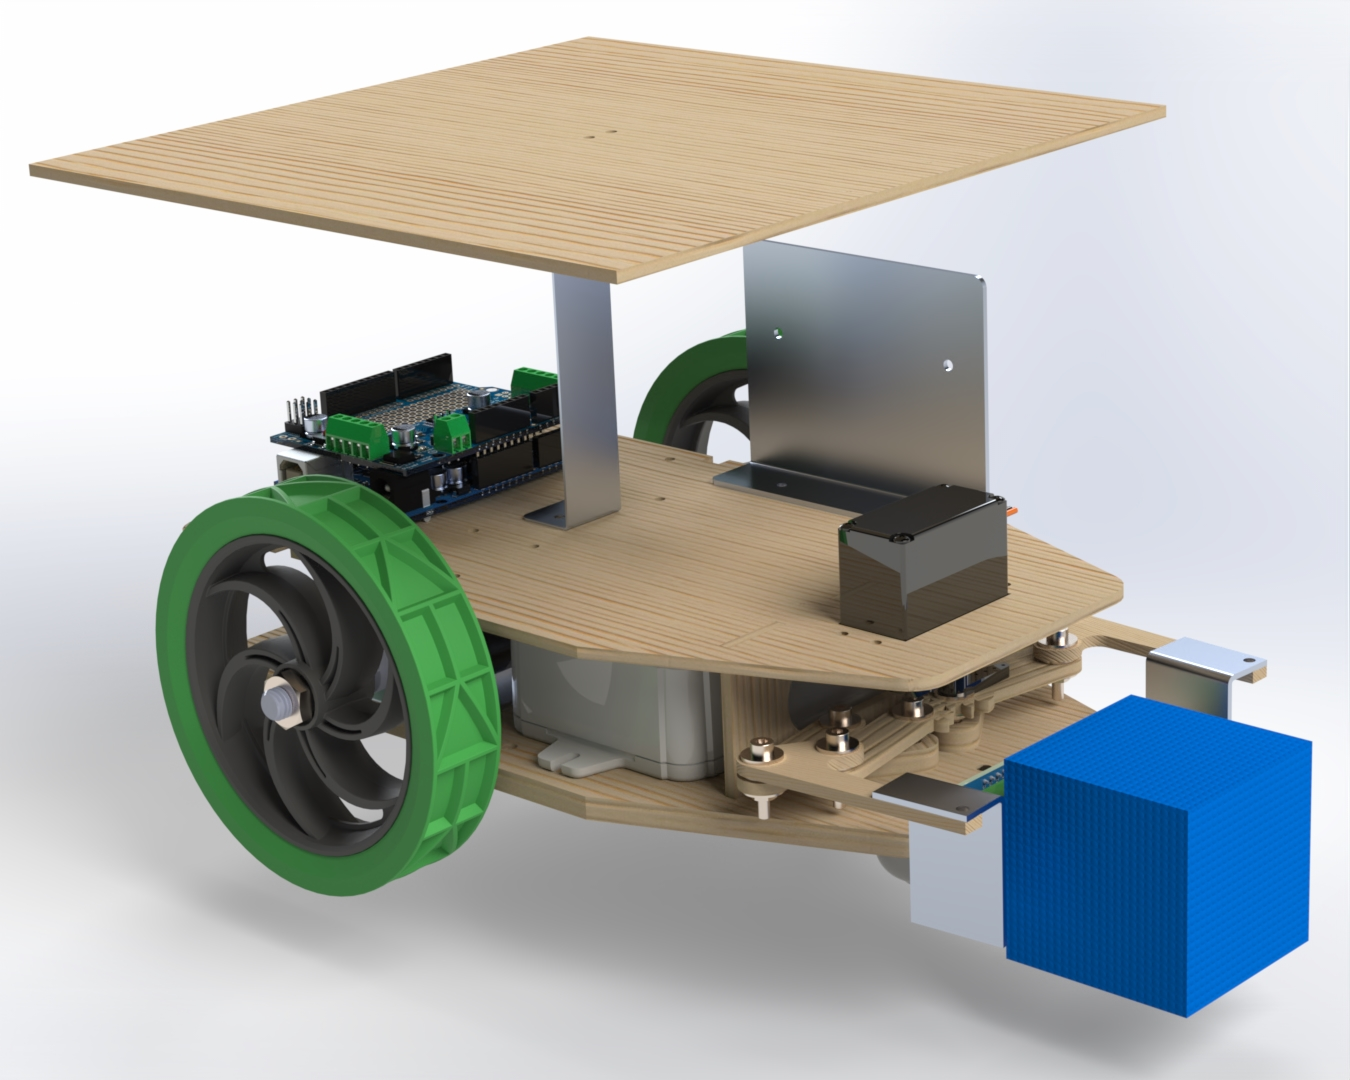
\includegraphics[width=0.8\textwidth]{assets/isometric.jpg}
    \label{fig:isometric}
    \caption{Isometric Render}
\end{figure}

\begin{figure}[H]
    \centering
    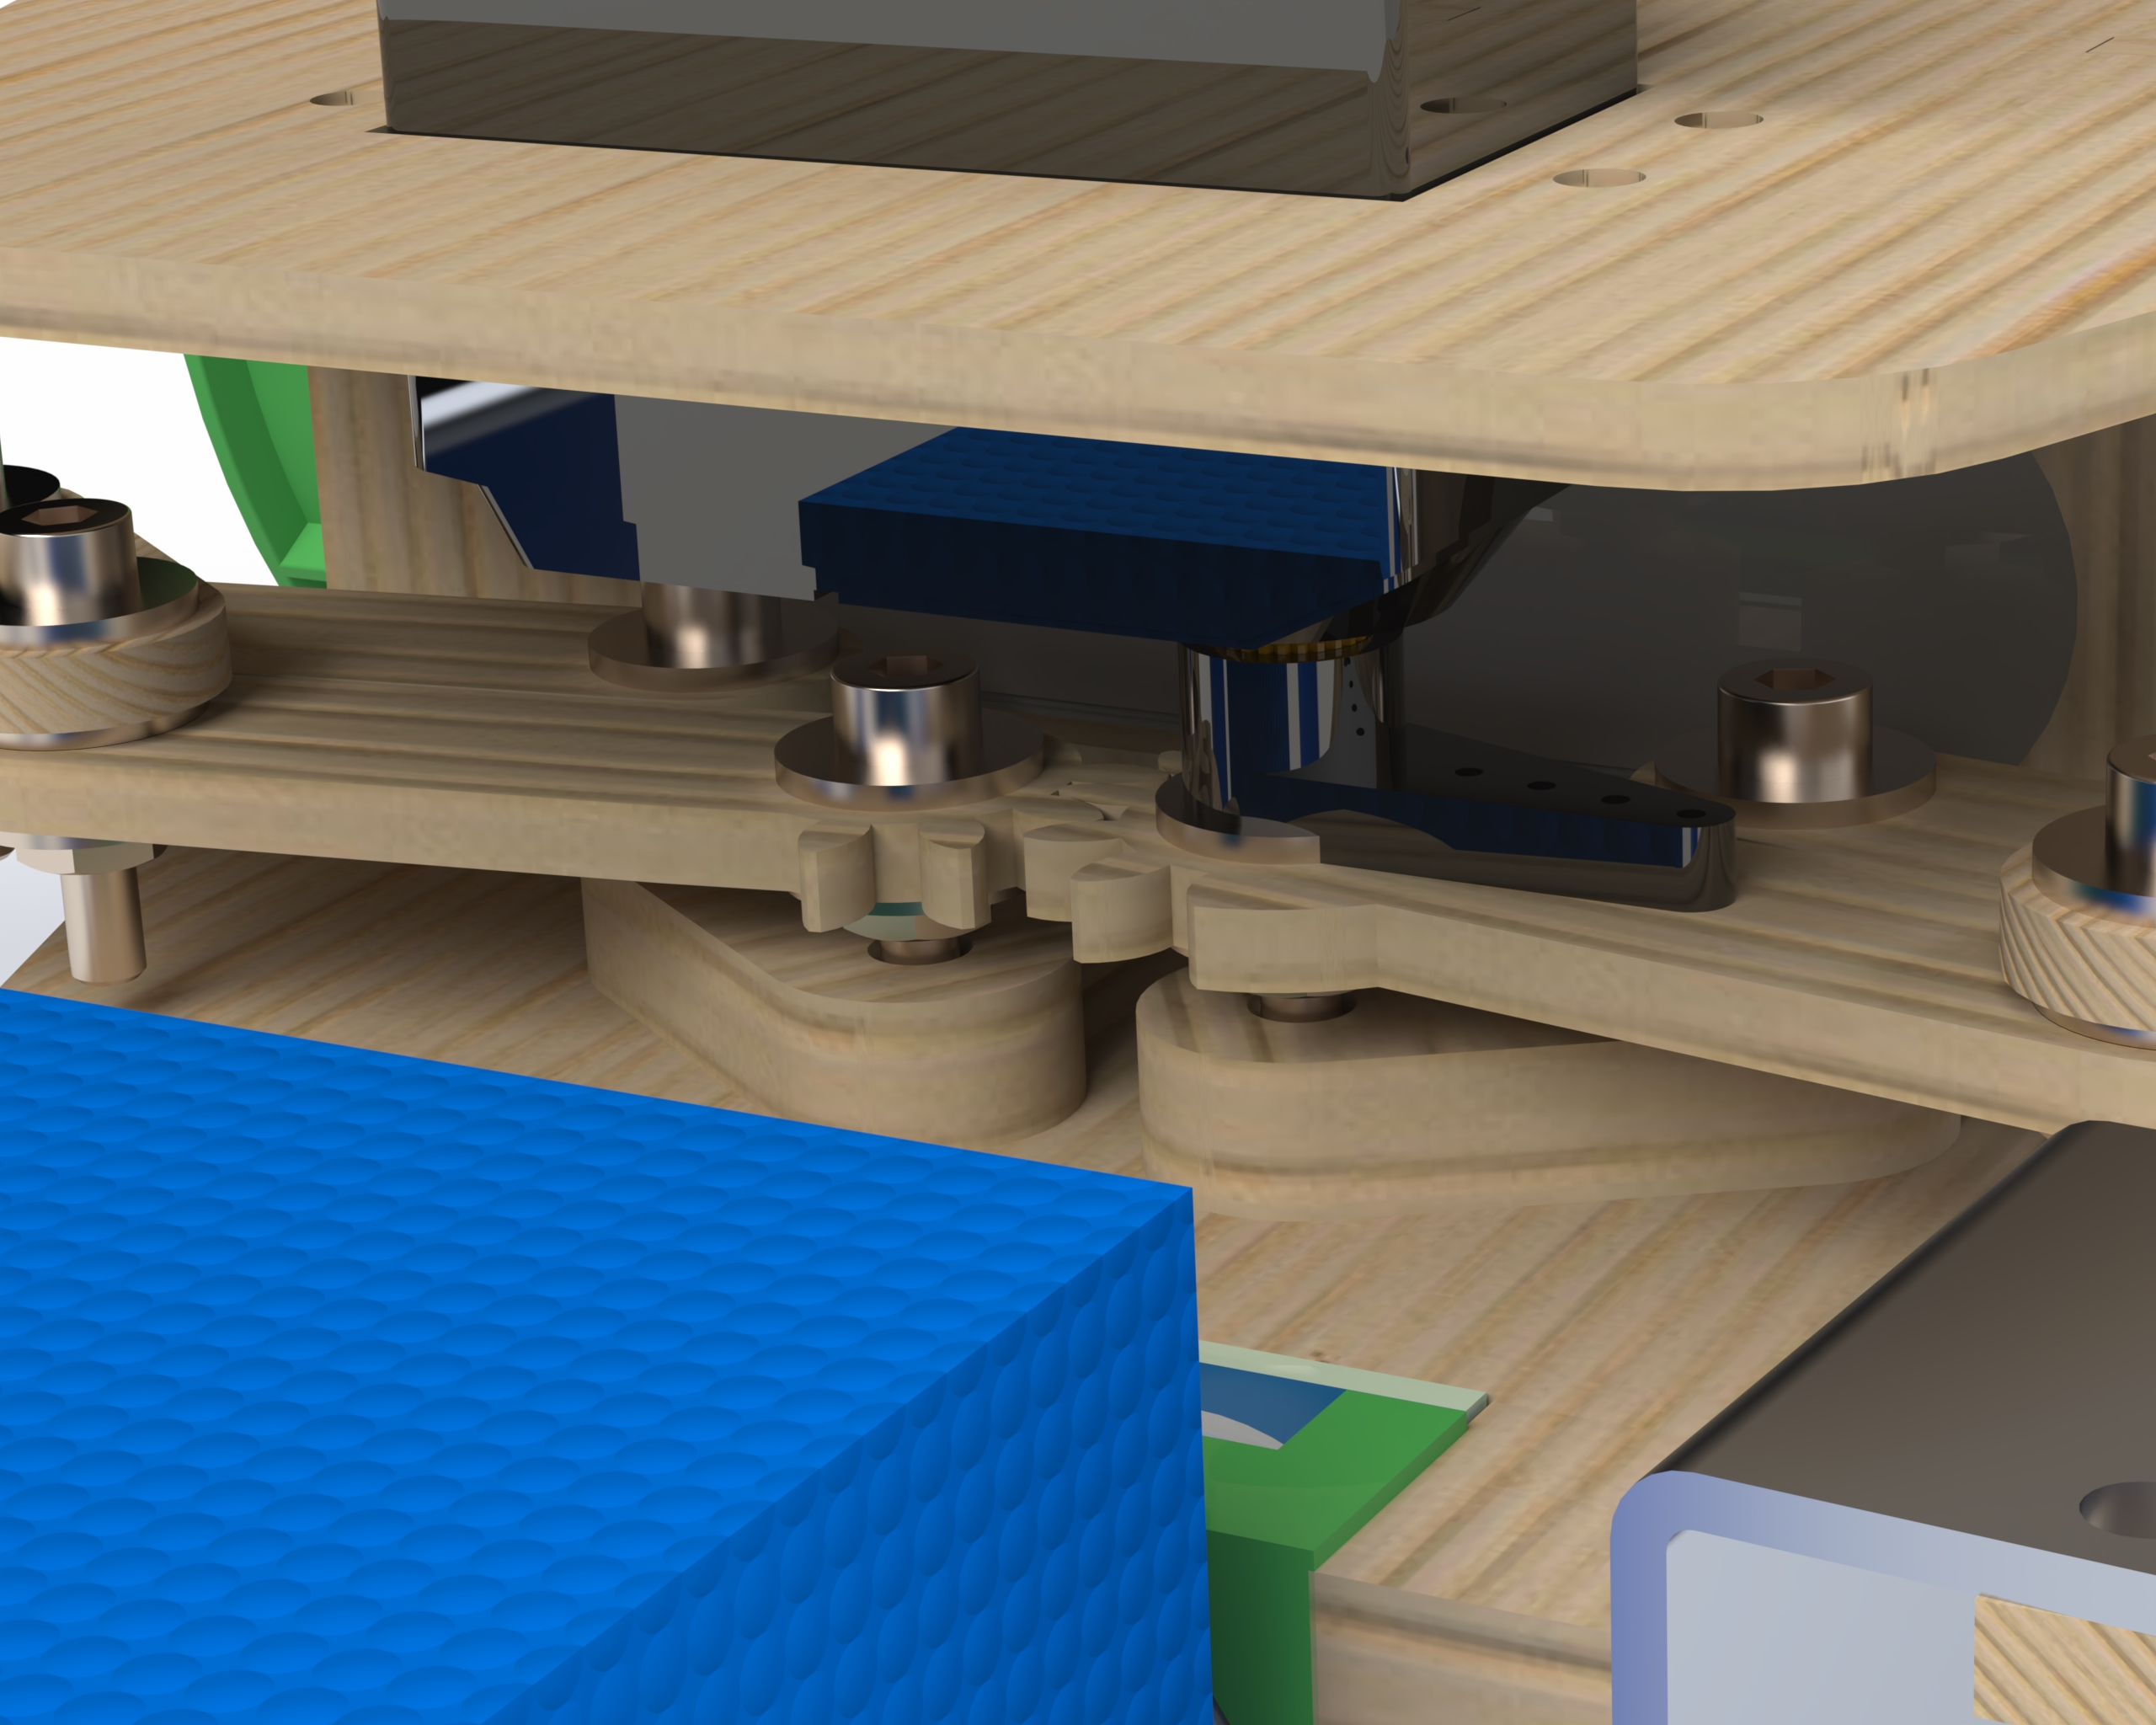
\includegraphics[width=0.8\textwidth]{assets/grabber_render.jpg}
    \label{fig:grabber_render}
    \caption{Grabber Render}
\end{figure}

\end{document}
